\documentclass[tikz,border=2.5mm,svgnames]{standalone}
\usepackage{tikz}
\usepackage{xcolor}
\usepackage{xifthen}
\usetikzlibrary{arrows.meta}
\usetikzlibrary{calc}
\begin{document}

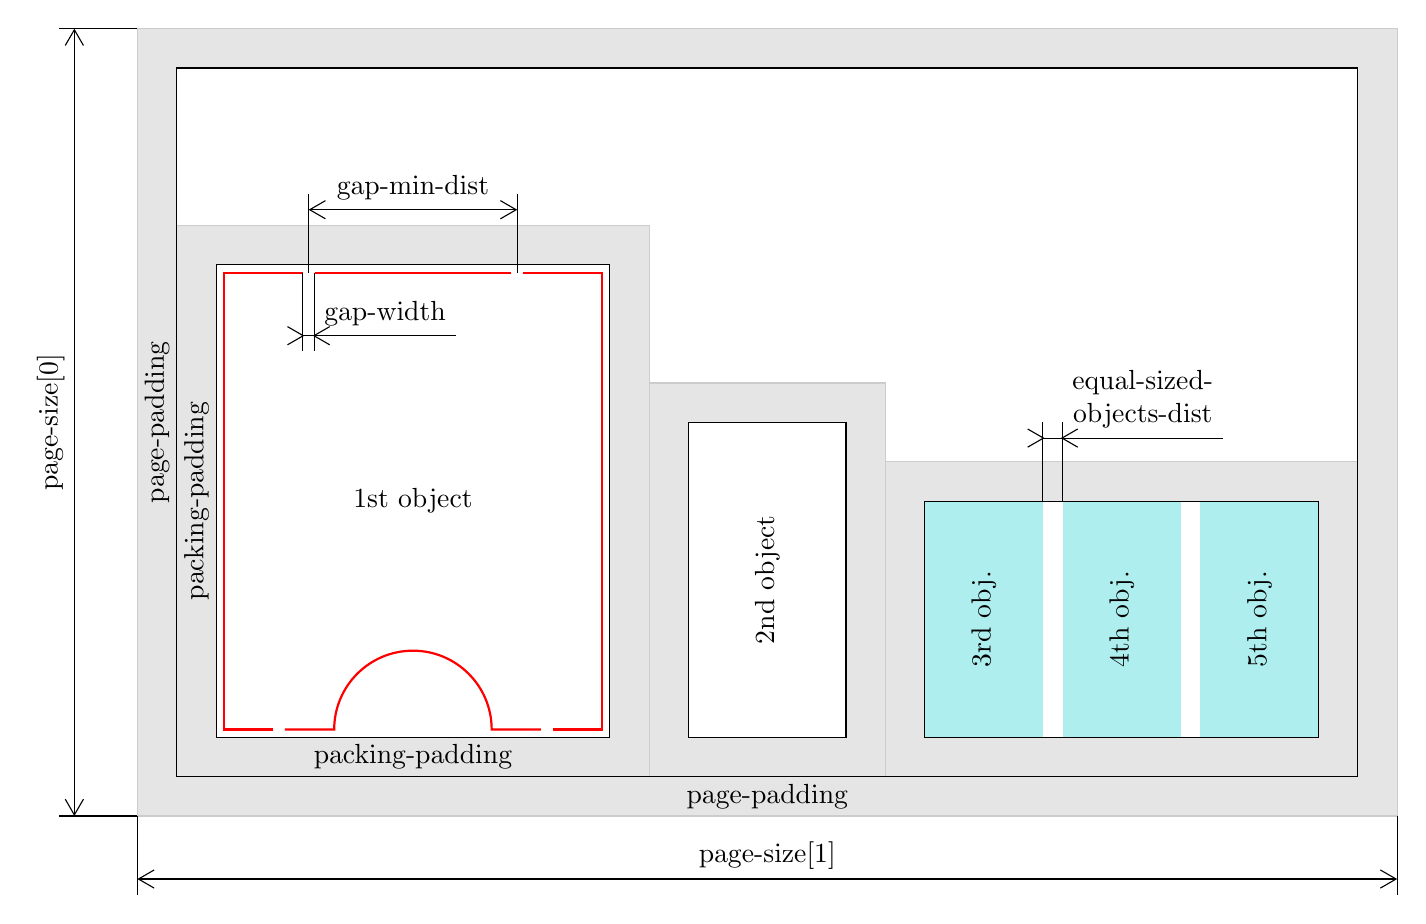
\begin{tikzpicture}[ar/.tip={Straight Barb[angle'=60,length=2mm]}]

\newcommand{\myframe}[5]{
    \coordinate (a) at (0,0);
    \coordinate (b) at (#1,#2);
    \coordinate (c) at ($(a)+(.5,.5)$);
    \coordinate (d) at ($(b)-(.5,.5)$);

    \fill [even odd rule,black!10] (a) rectangle #3 (b) (c) rectangle (d);

    \draw [black!20,thin] (a) rectangle (b);

    #4

    \draw [black,thin] (c) rectangle (d);

    \ifthenelse{\isempty{#5}}{}{
        \path let \p1 = (b) in node [yshift=.25cm] at ($(a)!.5!(\x1,0)$) {#5};
        \path let \p1 = (b) in node [xshift=.25cm,rotate=90] at ($(a)!.5!(0,\y1)$) {#5};
    }
}

\newcommand{\dimline}[4]{
    \begin{scope}[black,thin]
        \coordinate (f) at #1;
        \coordinate (s) at #2;

        \coordinate (v) at ($(f)-(s)$);

        \draw (f) -- ($(f)!1cm!90:(s)$) coordinate (aa);
        \draw (s) -- ($(s)!1cm!270:(f)$) coordinate (bb);
        \draw [draw=none] let \p1=(v), \n1={{veclen(\x1,\y1)}}, \n2={acos(-\x1/\n1)} in ($(f)!.8cm!(aa)$) coordinate (cc) -- ($(s)!.8cm!(bb)$) coordinate (dd) \pgfextra{\xdef\l{\n1}} \pgfextra{\xdef\ang{\n2}};

        \ifthenelse{\lengthtest{\l>1cm}}{
            \draw [ar-ar] (cc) -- (dd) node [midway,above,sloped] {#3};
        }{
            \draw [{ar[reversed,sep=-2mm]}-{ar[reversed,sep=-2mm]}] (cc) -- (dd);

            \ifthenelse{\equal{#4}{star}}{
                \node [anchor=south west,align=center,rotate=180-\ang] at (cc) (ee) {#3};
                \draw let \p1=($(ee.east)-(ee.west)$),
                    \n1={veclen(\p1)} in (cc) -- ($(dd)!\n1+\l!(cc)$);
            }{
                \node [anchor=south west,align=center,rotate=\ang] at (dd) (ee) {#3};
                \draw let \p1=($(ee.east)-(ee.west)$),
                    \n1={veclen(\p1)} in (dd) -- ($(cc)!\n1+\l!(dd)$);
            }

        }
    \end{scope}
}

\begin{scope}[shift={(.5,.5)}]
    \myframe{6}{7}{
        node [black] {1st object}
    }{
        \begin{scope}[shift={(.6,.6)},red,thick]
            \draw (1,5.8) -- ++(-1,0) -- ++(0,-5.8) -- ++(.625,0) coordinate (end);
            \draw ($(end)+(.15,0)$) -- ++(.625,0) arc [start angle=180,delta angle=-180, radius=1] -- ++(.625,0) coordinate (end);
            \draw ($(end)+(.15,0)$) -- ++(.625,0) -- ++(0,5.8) -- ++(-1,0) coordinate (end);
            \draw ($(end)-(.15,0)$) -- ++(-2.5,0) coordinate (end);

            \dimline{(1+.075,5.8)}{(3.8-.075,5.8)}{gap-min-dist}{};

            \dimline{(1.15,5.8)}{(1,5.8)}{gap-width}{star};
        \end{scope}

    }{packing-padding};
\end{scope}

\begin{scope}[shift={(6.5,.5)}]
    \myframe{3}{5}{
        node [black,rotate=90] {2nd object}
    }{}{};
\end{scope}

\begin{scope}[shift={(9.5,.5)}]
    \myframe{6}{4}{}{
        \begin{scope}[shift={(.5,.5)}]
            \fill [PaleTurquoise] (0,0) rectangle node [black,rotate=90] {3rd obj.} (1.5,3);
            \fill [PaleTurquoise] (1.75,0) rectangle node [black,rotate=90] {4th obj.} +(1.5,3);
            \fill [PaleTurquoise] (3.5,0) rectangle node [black,rotate=90] {5th obj.} +(1.5,3);

            \dimline{(1.5,3)}{(1.75,3)}{equal-sized-\\objects-dist}{};
        \end{scope}
    }{};
\end{scope}

\begin{scope}
    \myframe{16}{10}{}{}{page-padding};

    \dimline{(0,0)}{(0,10)}{page-size[0]}{};
    \dimline{(16,0)}{(0,0)}{page-size[1]}{};
\end{scope}

\end{tikzpicture}

\end{document}
